%%%%%%%%%%%%%%%%%%%%%%%%%%%%%%%%%%%%%%%%%%%%%%%%%%%%%%%%%%%%%%%%%%%%%%%%%%% 
% 
% Generic template for TFC/TFM/TFG/Tesis
% 
% By:
% + Javier Macías-Guarasa. 
% Departamento de Electrónica
% Universidad de Alcalá
% + Roberto Barra-Chicote. 
% Departamento de Ingeniería Electrónica
% Universidad Politécnica de Madrid   
% 
% Based on original sources by Roberto Barra, Manuel Ocaña, Jesús Nuevo,
% Pedro Revenga, Fernando Herránz and Noelia Hernández. Thanks a lot to
% all of them, and to the many anonymous contributors found (thanks to
% google) that provided help in setting all this up.
% 
% See also the additionalContributors.txt file to check the name of
% additional contributors to this work.
% 
% If you think you can add pieces of relevant/useful examples,
% improvements, please contact us at (macias@depeca.uah.es)
% 
% You can freely use this template and please contribute with
% comments or suggestions!!!
% 
%%%%%%%%%%%%%%%%%%%%%%%%%%%%%%%%%%%%%%%%%%%%%%%%%%%%%%%%%%%%%%%%%%%%%%%%%%% 

\chapter{Exploring GAN for Vehicle Motion Prediction}
\label{cha:exploring_gan_for_vehicle_mp}

\begin{FraseCelebre}
	\begin{Frase}
		El mundo no es todo alegría y color, \\
		es un lugar terrible y por muy duro que seas \\
		es capaz de arrodillarte a golpes \\
		y tenerte sometido a golpes permanentemente \\
		si no se lo impides. \\
		Ni tú ni yo ni nadie golpea mas fuerte que la vida. \\
		Pero no importa lo fuerte que golpeas, \\
		sino lo fuerte que pueden golpearte \\
		hay que soportar sin dejar de avanzar. \\
		¡Así es como se gana!
	\end{Frase}
	\begin{Fuente}
		Discurso de Rocky a su hijo \\
		Rocky Balboa
	\end{Fuente}
\end{FraseCelebre}

\section{Introduction}
\label{sec:5_introduction}

Despite the fact that SmartMOT illustrates a simple-yet-powerful tracking and prediction pipeline, traditional methods for \ac{MP} in the field of \ac{AD} are based on physical kinematic constraints and road map information with handcrafted rules. Though these approaches are sufficient in many simple situations (\ie \ vehicles moving in constant velocity or straightforward intersections), they fail to capture the rich behavior strategies and interaction in complex scenarios, in such a way they are only suitable for simple prediction scenes and short-time prediction tasks \cite{huang2022survey}. In that sense, as commented in Chapter \ref{sec:2_dl_based_mp}, recently \ac{DL} based methods have dominated this task and they usually follow an encoder-decoder paradigm. 

The main challenge in the \ac{MP} is the human driver behaviour can neither be modeled and consequently predicted properly, specially in negotiating situations \cite{gomez2021train} \cite{mercat2020multi} with many participants where considering agent-environment/agent-agent interactions \cite{sadeghian2019sophie} plays a determinant role. Then, resulting trajectories may not be necessarily feasible, not covering the full spectrum of possible trajectories that a vehicle can take. In that sense, a more natural way of capturing the feasible directions \cite{dendorfer2020goal} is to first compute a set of intermediate target points from a distribution of acceptable positions. 

In this chapter we explore the influence of attention mechanisms in generative models, in particular based on \ac{GAN} \cite{goodfellow2020generative}, to carry out the task of motion prediction. Our model considers both physical context, computing acceptable target points from the driveable area around the target agent, and social context, \ac{LSTM} \cite{hochreiter1997long} based encoder as input to a Multi-head self-attention module, as input of our generator, which combines the scene understanding around the agent vehicle (target agent to predict its trajectory) and the corresponding noise vector associated to generative models to compute the trajectories using a LSTM decoder, as illustrated in Figure \ref{fig:chapter_5_GAN/ITSC_2022}. In this context, the discriminator is applied in order to force the generator model to produce more realistic samples (\ie \ trajectories), hence, to improve the performance. 

Prior knowledge on \ac{MP} in pedestrian datasets like ETH \cite{pellegrini2009you} or UCY \cite{lerner2007ucydata} usually focuses on deep methods such as \acp{LSTM} \cite{hochreiter1997long} and \acp{GAN} \cite{goodfellow2020generative}. SocialLSTM \cite{alahi2016social} proposes an \ac{LSTM}-based model that can jointly predict the paths of all agents in the scene taking into account the common sense rules and social conventions using a social-pooling module. SocialGAN \cite{gupta2018social} enhances SocialLSTM with a generative adversarial framework, introducing a variety loss that encourage the network to cover the space of plausible paths and proposing a novel pooling global social pooling vector that encodes the subtle cues for all agents involved in the scene. SoPhie \cite{sadeghian2019sophie} considers not only the path history of all agents but also the physical context information (captured by a top-view static image, computing salient regions of the scene), combining physical and social attention mechanisms in order to help the model knows what to extract and where to focus. Goal-GAN \cite{dendorfer2020goal} predicts the most likely goal points of the agent of interesting, estimating a set of trajectories towards these potential future candidates using both physical and social context, as proposed by \cite{sadeghian2019sophie}. On the other hand, in the context of vehicle prediction \cite{chang2019argoverse, caesar2020nuscenes}, prior information takes more importance regarding the risk at certain velocities in urban / highway environments in order to perform safe navigation.

As stated in Chapter \ref{sec:2_dl_based_mp}, HD maps have been widely adopted to provide a preliminary raw physical context and then apply data-driven approaches. Recent learning-based approaches \cite{hong2019rules, casas2018intentnet}, which present the benefit of having probabilistic interpretations of different behaviour hypotheses, require to build a representation to encode the trajectory and map information. \cite{hong2019rules} assumes that detections around the vehicle are provided and focuses its work on behaviour prediction by encoding entity interactions with ConvNets. Intentnet \cite{casas2018intentnet} proposes to jointly detect traffic participants (mostly focused on vehicles) and predict their trajectories using raw LiDAR pointcloud and rendered HD map information. PRECOG \cite{rhinehart2019precog} aims to capture the future stochasiticity by flow-based generative models. Furthermore, MultiPath \cite{chai2019multipath} uses ConvNets as encoder and adopts pre-defined trajectory anchors to regress multiple possible future trajectories. 

Furthermore, as commented in previous sections, in a similar way to humans that pay more attention to close obstacles, people walking towards them or upcoming turns rather than considering the presence of people or building far away, the perception layer of a self-driving car must be modelled to focus more on the more relevant features of the scene. Social Attention is a mechanism that allows selective interactions within relevant agents. SoPhie \cite{sadeghian2019sophie} computes a different context vector for each agent, in such a way other agents features are sorted in terms of their relative distance to the agent of interest. Then, a soft attention mechanism is used to compute a context feature vector, which represents the social context. Nevertheless, a fixed size ($N_{\text{max}}$ agents) list that considers the context of all agents is sensitive to small variations \cite{mercat2020multi} of other agents positions. In that sense, SocialWays \cite{amirian2019social} presents a hand-crafted relative geometric feature to produce a set of normalized weights, in such a way the context vector represents a convex sum of other feature vectors (context of each agent) that is invariant to the ordering. 

However, these attention mechanisms were not designed to model complex interactions, no more than angles and distances due to the inherent problem of pedestrian prediction, in such a way we must find this challenging interactions in the vehicle motion prediction task to account for specific behaviours like overtaking, Adaptive Cruise Control (ACC), emergency braking or yielding. GRIP \cite{li2019grip} proposes a graph representation of vehicle neighbours, taking into account local interactions with vehicles that are closer to the target agent than a threshold distance \textit{d}.

\cite{vemula2018social} use a dot product attention module (inspired from the attention mechanism proposed by \cite{vaswani2017attention} for sentence translation), allowing joint forecast of every agent in the scene without spatial limitations, considering long range interactions regardless the ordering of the input vehicles tracks and the number of vehicles. Moreover, \cite{vemula2018social} combines this dot product with a spatio-temporal graph representation to take into account temporal and spatial dependencies of the agents, such as their absolute/relative positions and time step movements. \cite{mercat2020multi} present a multi-head extension of this dot attention mechanism, where each agent is embedded by means LSTMs before computing the dot product attention in order to produce social interactions. 

\section{Attention-based GAN}
\label{sec:5_attention_gan}

In this work, we aim to develop a model \cite{gomez2022exploring} that can successfully predict plausible future trajectories in the context of vehicle prediction, taking into account not only the past trajectory of the corresponding agent but also the HD map information to compute a set of acceptable target points representing the physical constraints for our problem.

When vehicles drive through a traffic scenario, they usually aim to reach partial goals, depending on their predefined navigation route and scene context (both physical and social), until they finally arrive at their final destination. Formally, given a certain goal, vehicles must face different traffic rules and other agents along their way to reach their final destination. Regarding this, our model computes both the social context and acceptable target points for the corresponding agent given its past trajectory and then generates plausible trajectories towards the estimated goals. As illustrated in Figure \ref{fig:chapter_5_GAN/ITSC_2022}, our model consists of three main blocks:

\begin{itemize}
	
	\item \textbf{Target Points Extractor}: Combines HD Map information and dynamic features of the target agent (speed and orientation) to generate acceptable target points in the driveable area.
	\item \textbf{Attention module}: Computes the agents dynamic features recursively by means a \ac{LSTM} unit and capture complex social interactions among agents by means of Multi-Head Self Attention.
	\item \textbf{\ac{GAN} module}: Given the target points and highlighted social features, this module generates plausible and realistic trajectories using a LSTM based decoder, which represents the generator. Discriminator is applied to enhance the performance of the generator by forcing it to compute more realistic predictions.
	
\end{itemize} 

\begin{figure}[h] 
	\centering
	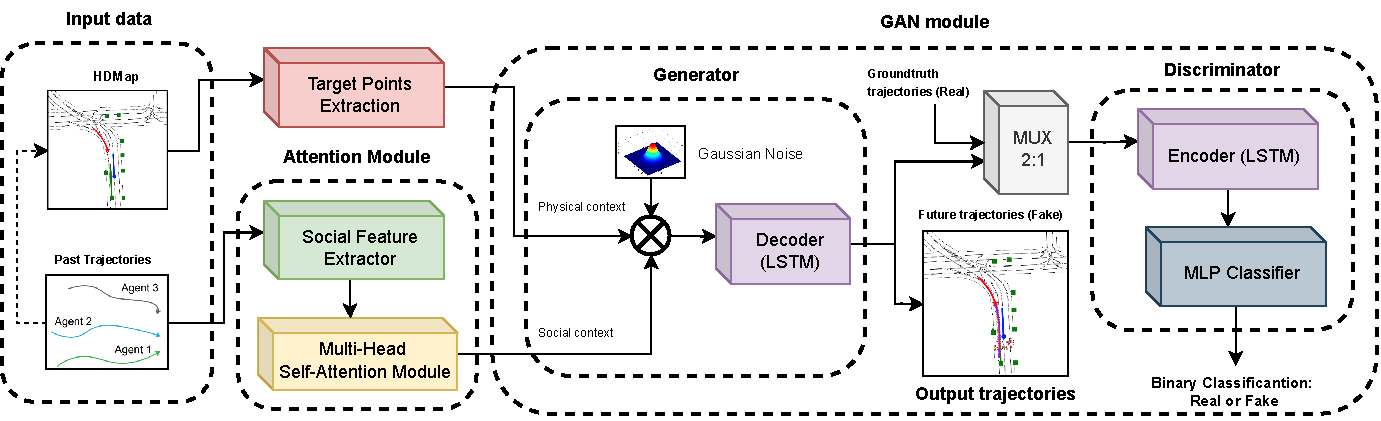
\includegraphics[width=\textwidth]{chapter_5_GAN/ITSC_2022.pdf}
	%\captionsetup{justification=justified}
	\caption{Overview of our Attention-based Generative model}
	\label{fig:chapter_5_GAN/ITSC_2022}
\end{figure}

Figure \ref{fig:chapter_5_GAN/ITSC_2022} illustrates an overview of our model. Next, we describe the different blocks of our model.

\subsection{Target points extraction}
\label{subsec:5_target_points_extraction}

Multiple approaches have tried to predict realistic trajectories by means of learning physically feasible areas as heatmaps or probability distributions of the agent future location \cite{dendorfer2020goal, sadeghian2019sophie, gilles2021home}. These approaches require either a top-view RGB BEV image of the scene, or a HD Map with exhaustive topological, geometric and semantic information (commonly codified as channels). This information is usually encoded using a CNN and fed into the model together with the social agent information \cite{dendorfer2020goal, sadeghian2019sophie, gao2020vectornet}.

In our model, we propose to estimate the range of motion (360º) using a minimal HD Map representation that includes only the feasible area, where we can discretize the feasible area $\mathcal{F}$ (represented by a discrete grid of the \textit{width} x \textit{height} BEV map image where the pixels are driveable) as a subset of $r$ randomly sampled points $\{p_0 , p_1 ... p_r\}$ from such area in the map (easy to extract from a 1-channel binarized HD image) considering the orientation and velocity in the last observation frame for the agent. This step can be considered as pre-processing of the HD Map, therefore the model never sees the HD map image nor the whole graph of nodes. 

\begin{figure}[!ht]
	\centering
	\begin{subfigure}{0.24\textwidth}
		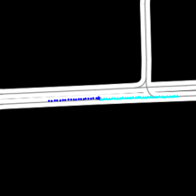
\includegraphics[width=\textwidth]{chapter_5_GAN/filtering_process_1_agent_trajectory.png}	
		\caption{}
	\end{subfigure}
	\hfill
	\begin{subfigure}{0.24\textwidth}
		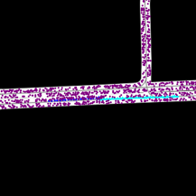
\includegraphics[width=\textwidth]{chapter_5_GAN/filtering_process_2_feasible_area_discretization.png}
		\caption{}
	\end{subfigure}
	\hfill
	\begin{subfigure}{0.24\textwidth}
		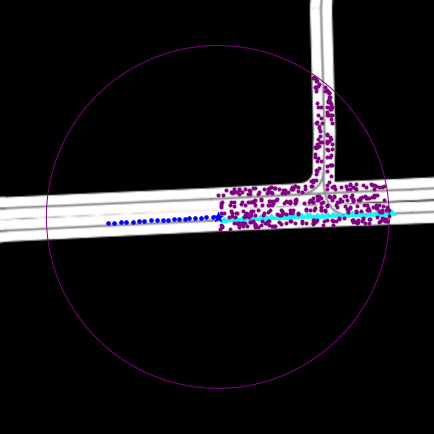
\includegraphics[width=\textwidth]{chapter_5_GAN/filtering_process_3_non_holonomic_filter.png}
		\caption{}
	\end{subfigure}
	\hfill
	\begin{subfigure}{0.24\textwidth}
		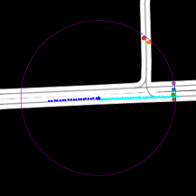
\includegraphics[width=\textwidth]{chapter_5_GAN/filtering_process_4_multimodal_clustering.png}
		\caption{}
	\end{subfigure}
	\captionsetup{justification=justified}
	\caption[Target Points Estimation from the Feasible area process]{Target Points Estimation from the Feasible area process: (a): Agent Past Trajectory (\textcolor{blue}{past observations} and \textcolor{aqua}{ground-truth}), (b) Feasible area discretization (random points in the driveable area), (c) Non-holonomic-based dynamic filter (both angle and velocity), (d) Multimodal clustering to get the final proposals}
	\label{fig:chapter_5_GAN/target_points_extraction}
\end{figure}

Figure \ref{fig:chapter_5_GAN/target_points_extraction} summarizes step-by-step the whole process. First, we calculate the driveable area (white area in Figure \ref{fig:chapter_5_GAN/target_points_extraction}) around the vehicle considering a hand-defined \textit{d} threshold.

Then, we consider the dynamic features of the agent of interest in the last observation frame $t_{obs}$ to compute acceptable target points in local coordinates. As we will detail in future sections, the Argoverse 1 Motion Forecasting dataset focuses on estimating the future prediction of a particular target agent. On top of that, the aforementioned dynamic features (orientation and velocity) are not provided, in such a way they must be calculated. Since the trajectory data are noisy with tracking errors, as expected from a real-world dataset, simply interpolating the coordinates between consecutive time steps, assuming constant frequency, results in noisy estimation. Then, in order to estimate the orientation and velocity of the target agent in the last observation frame $t_{obs}$, we compute a vector for each feature given:

\begin{equation}
	\begin{split}
		\theta_{i}=\arctan{(\frac{y_{i}-y_{i-1}}{x_{i}-x_{i-1}})} \\
		v_{i}=\frac{X_{i}-X_{i-1}}{t_{i}-t_{i-1}} 
	\end{split}
\end{equation}
 
where $X_{i}$ represents the 2D position of the agent at each observed frame $i$ as state above. Once both vectors are computed, we obtain a smooth estimation as proposed by \cite{tang2021exploring} of the heading angle (orientation) and velocity by assigning less importance (higher forgetting factor) to the first observations, in such a way immediate observations are the key states to determine the current spatio-temporal variables of the agent, as depicted in Equation \ref{eq:5_dynamic_feats_last_observation_frame}, which applies to both the orientation and velocity vector: 

\begin{equation}
	\hat{\psi}_{T_h} = \sum_{t=0}^{T_h}\lambda^{T_h - t}\psi_t
	\label{eq:5_dynamic_feats_last_observation_frame}
\end{equation}

where $T_h$ is the number of observed frames, $\psi_t$ is the estimated orientation/velocity at the $t_{i}$ frame, $\lambda\in(0, 1)$ is the forgetting factor, and $\hat{\psi}_{t_obs}$ is the smoothed orientation/velocity estimation at the last observed frame. After estimating these variables, we calculate the range of motion around the target agent as a circle with radius: $H * \psi_{v}$ where $\psi_{v}$ is the estimated velocity using Equation \ref{eq:5_dynamic_feats_last_observation_frame} and $H=3$ is the time-horizon of 3s. After that, we randomly sample $r$ points $p \in \mathcal{F}$ in this range considering a constant velocity model during the prediction horizon and the estimated orientation, assuming non-holonomic constraints \cite{triggs1993motion}, which are inherent of standard road vehicles, that is, the car has three degrees of freedom, its position in two axes and its orientation, and must follow a smooth trajectory in a short-mid term prediction. Finally, we estimate $k$ target points (one per mode required in the future prediction) by means of the k-means \cite{ahmed2020k} clustering algorithm. 

This clustering method, originally from signal processing, that aims to partition n observations into k clusters in which each observation belongs to the cluster with the nearest mean (cluster centers or cluster centroid), serving as a prototype of the cluster. In this particular model, we focus on unimodal prediction, that is, the model must reason the most plausible future trajectory based on the agents past observations, attention-based social interaction and target points as physical context.

This representation not only reunites information about the feasible area around the agent, but also represents potential target points \cite{dendorfer2020goal} (\ie \ potential destinations or end-of-trajectory points for the agents). Moreover, this information is \textit{"cheap"} and \textit{interpretable}, therefore, we do not need further exhaustive annotations from the HD Map in comparison with other methods like HOME, which gets as input a 45-channel encoded map \cite{gilles2021home}.

We concatenate this information, as 2D vector $\mathcal{V}$, together with the model social context features to generate more realistic trajectories (see Figure \ref{fig:chapter_5_GAN/ITSC_2022}).

\subsection{Attention module}
\label{subsec:5_attention_module}

Multiple methods \cite{liang2020learning, schmidt2022crat} consider only the vehicles that are observable at \textit{t=0}, handling those agents that are not observed over the full sequence spectrum (observation length = \textit{$obs_{len}$} + prediction length = \textit{$pred_{len}$}) by concatenating a binary flag $b_i^t$ that indicates if the agent is padded or not. 

In our case, we consider the agents that have information over the full history horizon $T_h$ = \textit{$obs_{len}$} + \textit{$pred_{len}$} (\eg \ 5s timeframe for Argoverse) as relevant agents, reducing the number of agents to be considered in complex traffic scenarios. Nevertheless, instead of using the past $obs_len$ observations in map (global) coordinates for each agent marked as relevant, we transform to local (relative) coordinates by substracting the last observation of the target agent (considered as the origin of the scene) to the past trajectory of an agent to make the model translation-invariant given the local coordinates the scene. Then of using absolute 2D-BEV (\textit{xy} plane), the input for the agent \textit{i} is a series of relative displacements:

\begin{equation}
	\Delta \boldsymbol{\nu}^{t}_i = \boldsymbol{\nu}^{t}_i - \boldsymbol{\nu}^{t-1}_i
\end{equation}

Where $\boldsymbol{\nu}^{t}_i$ represents the state vector (in this case, \textit{xy} position of the agent \textit{i} at timestamp \textit{t}. % Once these displacements vectors are computed for each agent of the scenario, we embed them into a higher dimensional vector with a \ac{MLP}, which serves as input of the \ac{LSTM} unit, used as dynamic feature extractor to capture the speed and direction of the corresponding agent. Then, the hidden state of the LSTM ($h_{M\!E}$) is used by the MHSA module that learns complex social interactions while being invariant to their number and ordering, avoiding a fixed size ($N_{\text{max}}$ agents) list which would be sensitive to small variants in the agent positions.

Unlike other methods, we do not limit nor fix the number of agents per sequence. Given the relative displacements of all different agents, we model the past motion history by means of a single \ac{LSTM} (Social Feature Extractor in Figure \ref{fig:chapter_5_GAN/ITSC_2022}) is used to compute the temporal information of each agent in the sequence:

\begin{equation}
	out, \mathbf{h_{out}}, \mathbf{c_{out}} = \mathrm{LSTM}(\Delta \boldsymbol{\nu}^{obs_{len}}, \mathbf{h_{in}}, \mathbf{c_{in}})
\end{equation}

This \ac{LSTM}-based encoder shares the weights for all vehicles in the batch. The input hidden and cell vectors ($\mathbf{h_{in}}, \mathbf{c_{in}}$) are initialized with a tensor of zeros. $\Delta \boldsymbol{\nu}^{obs_{len}}$ represents the relative displacements over the whole past observations $obs_{len}$.

Then, after computing the social hidden state of each relevant agent in the traffic scenario, we aim to learn complex social interactions, where each agent of the scene should pay attention to specific features around it, while being invariant to their number and ordering, avoiding a fixed size ($N_{\text{max}}$ agents) list which would be sensitive to small variants in the agent positions.

To this end, we make use of a \ac{MHSA} module consists of several heads that given the encoded trajectories produces feature vectors that encode all pairwise relations among agents information, where the input (key, query, value) is the hidden vector ($\mathbf{h_{out}}$) of the previous Social Feature Extractor. The \ac{MHSA} module consists of several heads that given the encoded trajectories produces feature vectors that encode all pairwise relations among agents information, as stated in Chapter \ref{cha:theoretical_background}. %Implementation details are specified in Chapter \ref{sec:5_motion_prediction_datasets}.

\subsection{GAN module}
\label{subsec:5_gan_module}

To capture the stochastic nature of motion prediction, state-of-the-art methods leverage the power of generative models, such as Variational Autoencoders (VAEs) and Generative Adversarial Networks (GANs). In our work we use an adversarial framework in order to train our trajectory generator, responsible for generating physically and realistic feasible trajectories. In a GAN, the Generator (which after being trained will be the inference network) and Discriminator networks compete in a two-player min-max game \cite{goodfellow2020generative}, as observed in Equation \ref{eq:4_min_max_game}. While the generator aims at producing feasible trajectories, the discriminator learns to differentiate between fake and real samples, in other words, ground-truth (which are feasible by definition) and inferred trajectories, in such a way the tasks of the discriminator is to enhance the performance of the generator by forcing it to compute more realistic predictions, more and more similar to the ground-truth trajectory. As a result, the generator should be able to produce outputs which the discriminator cannot discriminate clearly, indicating that the output is realistic. 

\begin{eqnarray}
	\label{eq:4_min_max_game}
	&&\hspace{-10mm} \min_{Gen} \max_{Dis} V(Dis, Gen)=E_{X \sim p_{data}(X)}[\mbox{log} Dis(X,Y)] \nonumber \\
	&&\hspace{15mm} + E_{z \sim p_z(z)}[\mbox{log} (1 - Dis(X, Gen(X,z)))],
\end{eqnarray}

In the present case, the generator, also identified as the routing module, is represented by a decoder LSTM  ($LSTM_{gen}$) and the discriminator by a classifier LSTM ($LSTM_{dis}$) so as to estimate the temporally dependent future states. Similar to the conditional GAN proposed by \cite{sadeghian2019sophie}, the input to our generator is a concatenation of a noise vector $z$ sampled from a multi-variate normal distribution, being the physical context (goal points in relative coordinates in the last observation frame, $C_{Ph(i)}^{t_{obs}}$) and social context (interactions among agents, $C_{So(i)}^{1:t_{obs}}$) its conditions. Then, the generated future trajectory for a particular agent is modelled as Equation \ref{eq:4_gen_dec}:

\begin{eqnarray}
	\label{eq:4_gen_dec}
	& \hat{Y}_i^{t_{obs}:t_{pred}} = LSTM_{gen}\big(C_{Ph(i)}^{t_{obs}}; C_{So(i)}^{1:t_{obs}}; z\big)
\end{eqnarray}

On the other hand, the input of the discriminator is a randomly chosen trajectory sample from the either predicted future trajectory or ground-truth for the corresponding agent up to $t = t_{obs} + t_{pred}$ frame, i.e.  $T_i^{t_{obs}:t_{pred}}\sim p(\hat{Y}_i^{t_{obs}:t_{pred}},Y_i^{t_{obs}:t_{pred}})$.

\begin{eqnarray}
	\label{eq:4_dis}
	\hat{L}_{i}^{t_{obs}:t_{pred}} = LSTM_{dis}(T_i^{t_{obs}:t_{pred}})
\end{eqnarray}

Then, the discriminator returns a label $\hat{L}_{i}^{t_{obs}:t_{pred}}$ for the chosen trajectory indicating whether the trajectory is ground-truth (real) $Y_i^{t_{obs}:t_{pred}}$ or predicted (fake) $\hat{Y}_i^{t_{obs}:t_{pred}}$, being the labels 0 and 1 for fake and real trajectories respectively. Equation \ref{eq:4_dis} summarizes the discriminator working principles. 

\subsection{Losses}
\label{subsec:5_losses}

To train our \ac{GAN}-based model, we use the following losses:

\begin{eqnarray}
	\label{eq:obj}
	W^* =\operatorname*{argmin}_W \quad\mathbb{E}_{i,\tau}[\lambda_{gan} \mathcal{L}_{GAN}\big(\hat{L}_{i}^{t_{obs}:t_{pred}}, L_{i}^{t_{obs}:t_{pred}} \big)+ \nonumber\\
	\lambda_{ADE} \mathcal{L}_{ADE}(\hat{Y}_i^{t_{obs}:t_{pred}},Y_i^{t_{obs}:t_{pred}})+ \nonumber\\
	\lambda_{FDE} \mathcal{L}_{FDE}(\hat{Y}_i^{t_{obs}+t_{pred}},Y_i^{t_{obs}+t_{pred}})],
\end{eqnarray}
%
where $W$ is the collection of the weights of all networks used in our model and the different $\lambda$ represent the corresponding regularizers between these losses. As stated in Equation \ref{eq:4_min_max_game}, $\mathcal{L}_{GAN}$ represents the min-max game where the generator tries to minimize the function while the discriminator tries to maximize it. ADE loss function is commonly used to compute the average error between the predicted trajectories and the corresponding ground-truth. Moreover, we add FDE loss function to explicitly optimize the distribution towards the final real point.

\section{Experimental Results}
\label{sec:5_experimental_results}

\subsection{Dataset}
\label{subsec:5_dataset}

We evaluate this model on the well-established and public available Argoverse 1 Motion Forecasting dataset \cite{chang2019argoverse}, including the training, validation and testing subsets from its official website \cite{argobench}. 

As stated in Section \ref{subsec:2_argoverse_1}, it consists of 205942 training samples, 39472 validation samples and 78143 test samples. Each sample has a length of 5 seconds, with an observation window of 2 seconds and a prediction window of 3 seconds, including the corresponding labels of the agents ($AGENT$, as the target agent, $AV$, the vehicle that captures the scene and $OTHER$, representing the remaining relevant obstacles) and a global map from the cities of Pittsburgh and Miami. The sampling frequency is $10\mathrm{Hz}$. The main goal here is to predict the 3s future position of the target agent in the scene, which is supposed to be the vehicle that faces the most challenging traffic scenarios.

\subsection{Metrics}
\label{subsec:5_metrics}

Previous works \cite{chai2019multipath, mercat2020multi, sadeghian2019sophie} report the minimum Average Displacement Error ($\text{minADE}_K$), which averages the $L2$ distances between the ground truth and predicted output across all timesteps and minimum Final Displacement error ($\text{FDE}_K$), which computes the $L_{2}$ distance between the final points of the ground-truth and the predicted final position, taking the best $K$ trajectory sample of each agent compared to the ground truth. In this model, since we do not focus on multimodal prediction but on the predicting the most plausible unimodal trajectory, we use $K$ = 1 (unimodal case).

\subsection{Implementation details}
\label{subsec:5_implementation_details}

All local test were conducted in a PC desktop (AMD Ryzen 9 5900X, 32GB RAM with CUDA-based NVIDIA GeForce RTX 3090 24GB VRAM, Ubuntu 18.04).

We design our dataloader to sample in each batch a 30/70 proportion of straight and curved trajectories (regarding the target agent whole trajectory). We classify a trajectory as straight or curve estimating a first degree trajectory by means the RANSAC algorithm with the highest number of inliers (tolerance $t$ set to 2m, max trials=30, min samples=60 \% total observations). Then, if the actual trajectory presents 20 \% or more consecutive points further than $t$ with respect to the closest point of the fitted trajectory, the whole sequence is labelled as curve. We do this to focus in the training process in non-linear prediction, which represents one the key challenges in vehicle motion prediction. 

Regarding the ablation study, we train the different models for 150 epochs using the ADAM optimizer with learning rate $0.001$ and default parameters, linear LR Scheduler with factor $0.5$ decay on plateaus (5k iterations) and batch size $64$. The loss function is weighted by setting $\lambda_{gan}$=1.4, $\lambda_{ade}$=1 and $\lambda_{fde}$=1.5, giving more importance to the adversarial loss and the final displacement error. Similar to \cite{sadeghian2019sophie}, the LSTM encoder (attention block) encodes trajectories using a single layer MLP with an embedding dimension of 16. We set all LSTM units to have $32$ hidden dimensions. The number of target points is set also to 32 in order to compute the physical context. Moreover, in order to calculate these target points we consider the same prediction horizon $t_{pred}=3s$ to estimate the distance travelled assuming a constant velocity model. To make our model more robust to scene orientation, we augment the training data adding some white noise ($\mu=0, \sigma=0.25$, [m]) to the observation data, rotating the scene and also dropping and replacing (with their last frame) some observations of the past trajectory in order to make the trained model general enough so as to perform well on the unseen traffic scenarios in the split test which different scene geometries such as left/right turning or emergency braking.% and so forth and so on.

\subsection{Statistical study of the baseline in validation}
\label{subsec:5_target_agent_distribution}

In terms of validation, we conduct a statistical analysis for the ADE and FDE metrics, distinguishing the performance between straight and curved trajectories for our baseline model, \ie \ without considering target goals as map information and class balance in the batch. To this end, we make use of the Argoverse 1 validation set that consists of 31000 samples where 23012 and 7988 are straight and curved trajectories respectively given the RANSAC-based classification aforementioned. We show in Figure \ref{fig:chapter_5_GAN/boxplots} the boxplots for the ADE and FDE metrics. As stated before, our method, as most methods, struggles with curved trajectories, the overall ADE and FDE is "always" better for the straight trajectory cases. The median provides a robust estimator of our trajectories error. Note that we detected multiple outliers in our analysis, these are due to the unimodal nature of the model, unable to consider multiple possible hypotheses (multi-modal). 

\begin{figure}[!ht]
	\centering
	\setlength{\tabcolsep}{2.0pt}
	%\renewcommand{\arraystretch}{1.2}%
	\begin{tabular}{c}
		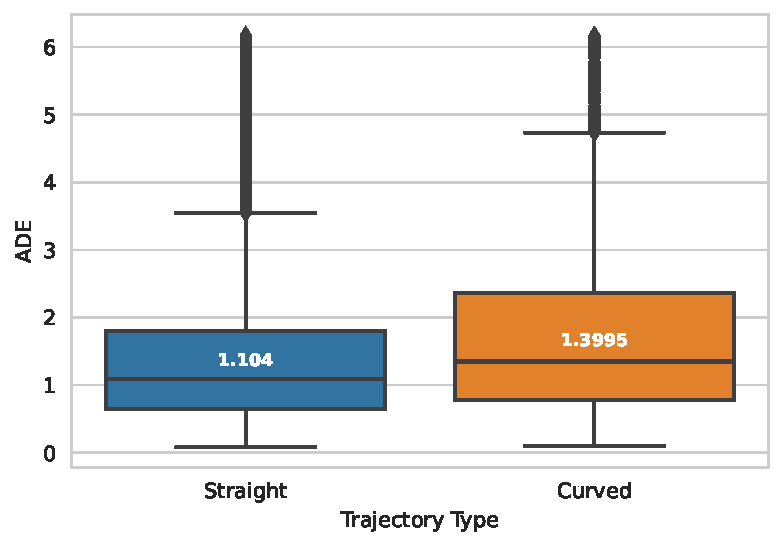
\includegraphics[width=0.4\linewidth]{chapter_5_GAN/ade_analysis.pdf} %\tabularnewline
		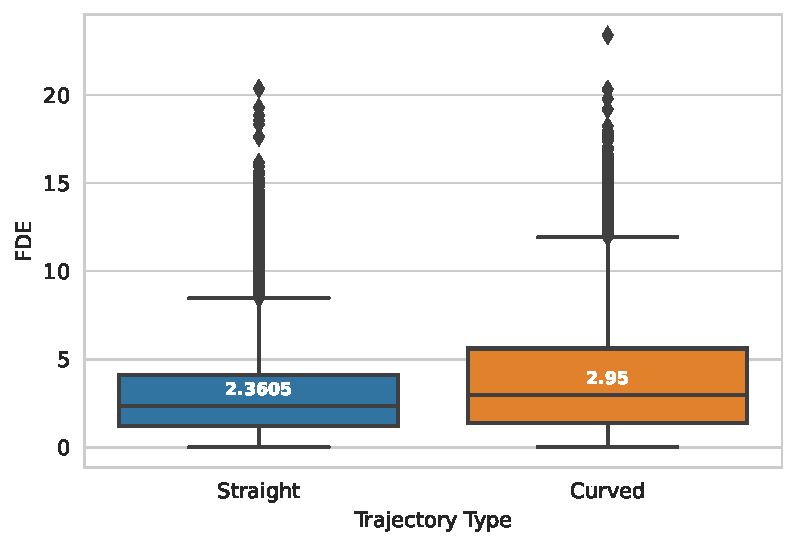
\includegraphics[width=0.4\linewidth]{chapter_5_GAN/fde_analysis.pdf}\tabularnewline
	\end{tabular}
	\caption[Statistical distribution on the Argoverse 1 validation set of regression metrics in straight and curved trajectories]{Statistical distribution on the Argoverse 1 validation set of regression metrics in straight and curved trajectories. We show the boxplots for ADE and FDE metrics. We distinguish between straight and curved trajectories. We highlight the median (Q2) in each boxplot.}
	\label{fig:chapter_5_GAN/boxplots}
\end{figure}

\subsection{Comparative with the state-of-the-art}
\label{subsec:5_model_results}

In this section, we perform an ablation study and compare our method performance against \ac{SOTA} methods on the Argoverse 1 Motion Forecasting benchmark test set. Table \ref{table:5_model_results_test} illustrates the comparison with some Argoverse baseline methods. Our baseline (*) is represented by the system pipeline illustrated in Figure \ref{fig:chapter_5_GAN/ITSC_2022}, that is, Attention-based \ac{GAN} with \ac{LSTM} as encoder-decoder, without target points extractor and class balance. We conduct an ablation study to observe the influence of incorporating target points and class balance to our baseline. As expected, by explicitly defining the locations an agent is likely to be at a fixed prediction horizon for a given input trajectory and scene geometry, we are able to improve our baseline. Additionally, since nonlinear trajectories are more challenging than standard straight trajectories, we also observe how enforcing the class balance (straight, curve) during training is able to improve performance.

\begin{table}[!h]
	\captionsetup{justification=justified}
	\caption[Ablation study of our Attention-based GAN unimodal pipeline, and comparison with other relevant methods on Argoverse 1 Motion Forecasting validation set]{Ablation study of our GAN-based unimodal pipeline, and comparison with other relevant methods on Argoverse 1 Motion Forecasting validation set. We can see the improvement using Target points (TP) and Class balance (CB). Our methods are indicated with $\dag$.}
	\begin{center}
		\begin{tabular}{ l | c | c }
			\toprule
			\textbf{Model} & \textbf{ADE (k=1) $\downarrow$} & \textbf{FDE (k=1) $\downarrow$} \\
			& [m] & [m] \\
			\midrule
			Constant Velocity \cite{chang2019argoverse} & 3.53 & 7.89 \\ 
			Argoverse Baseline (NN) \cite{chang2019argoverse} & 3.45  & 7.88 \\ 
			Argoverse Baseline (LSTM) \cite{chang2019argoverse} & 2.96  & 6.81 \\ 
			SGAN \cite{gupta2018social} & 3.61  & 5.39 \\ 
			TPNet \cite{fang2020tpnet} & 2.33  & 5.29 \\ 
			TPNet-map \cite{fang2020tpnet} & 2.33  & 4.71 \\ 
			Jean (1st) \cite{chang2019argoverse, mercat2020multi} & 1.74  & 4.24 \\ 
			\midrule 
			$\dag$ Baseline (*) & 1.98  & 4.47 \\ 
			$\dag$ + TP & 1.78  & 4.13 \\
			$\dag$ + CB & 1.82  & 4.09 \\
			$\dag$ + TP + CB & 1.67  & 3.82 \\
			\hline
		\end{tabular}
		\label{table:5_model_results_test}
	\end{center}
\end{table}

\subsection{Qualitative results}
\label{subsec:5_qualitative_results}

Figure \ref{fig:chapter_5_GAN/Unimodal_results} illustrates some qualitative results, all of them considering uni-modal prediction towards the pre-computed target points, meeting the physical and social constraints in the scenes. It can be clearly appreciated that a naive \ac{CTRV} model could not generalize in these situations, where the vehicle can describe a curved future trajectory given a predominant straight input trajectory and vice-versa. First and second rows show feasible predicted trajectories, whilst the third one shows interesting challenging scenarios in which our current approach is not able to properly reason due to the lack of reasoning and multi-modality (producing a set of K-trajectories towards the set of target points) is revealed, being situations in which predicting accurately the end-point is difficult, and this the \ac{FDE} is extremely high. 

In that sense, regarding the third row, left image shows how we compute an uni-modal prediction in the wrong direction of a split, even though target points are extracted very close to the ground-truth end point. Center image shows an extreme difficult situation, where the input trajectory is almost in the same place (probably the target agent was stopped in front a traffic light) whilst the ground-truth future trajectory is clearly an acceleration since the last observation frame. Finally, right image shows a deceleration because of the ahead obstacle whilst our model is not able to properly reason the presence of this obstacle in order to meet common sense safety constraints.

\begin{figure*}[!ht]
	\centering
	\setlength{\tabcolsep}{2.0pt}
	\begin{tabular}{cccc}
		\fbox{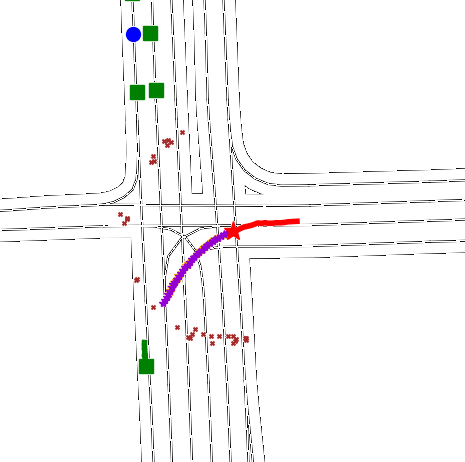
\includegraphics[width=0.32\linewidth]{chapter_5_GAN/qualitative/2044_unimodal.png}} &
		\fbox{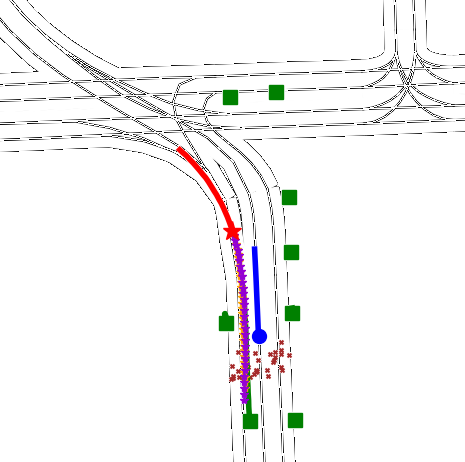
\includegraphics[width=0.32\linewidth]{chapter_5_GAN/qualitative/2079_unimodal.png}} &
		\fbox{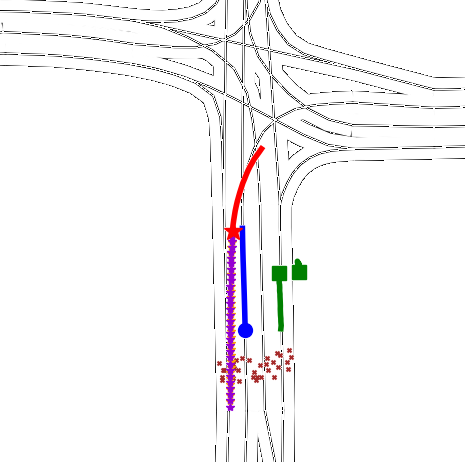
\includegraphics[width=0.32\linewidth]{chapter_5_GAN/qualitative/2117_unimodal.png}}
		\tabularnewline
		\fbox{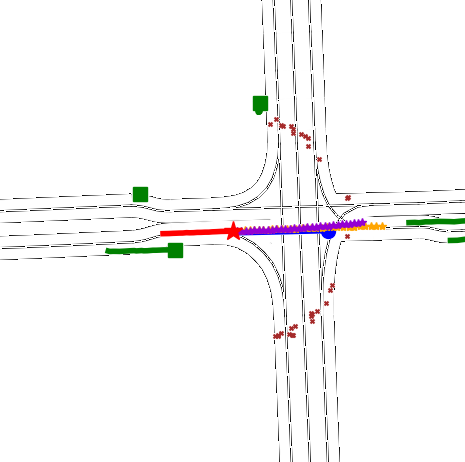
\includegraphics[width=0.32\linewidth]{chapter_5_GAN/qualitative/838_unimodal.png}} &
		\fbox{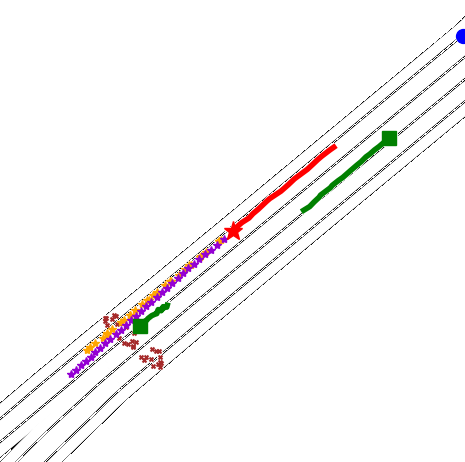
\includegraphics[width=0.32\linewidth]{chapter_5_GAN/qualitative/868_unimodal.png}} &
		\fbox{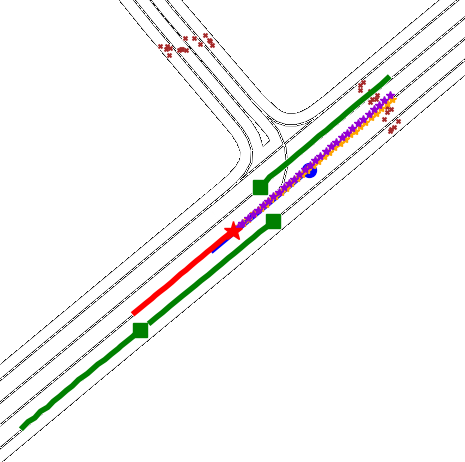
\includegraphics[width=0.32\linewidth]{chapter_5_GAN/qualitative/887_unimodal.png}}
		\tabularnewline
		\fbox{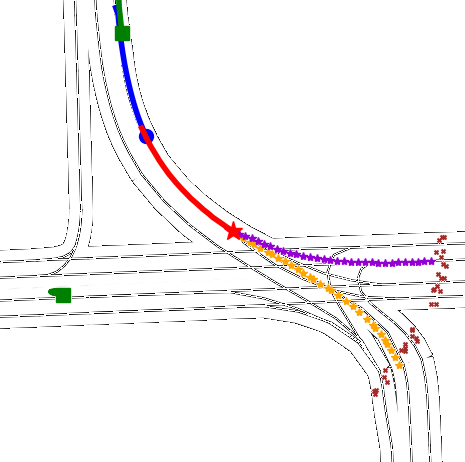
\includegraphics[width=0.32\linewidth]{chapter_5_GAN/qualitative/11_unimodal.png}} & 
		\fbox{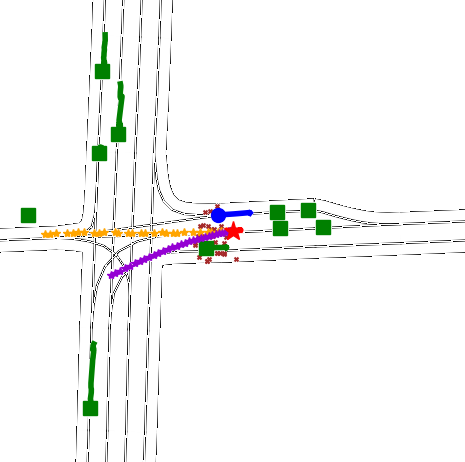
\includegraphics[width=0.32\linewidth]{chapter_5_GAN/qualitative/49_unimodal.png}} &
		\fbox{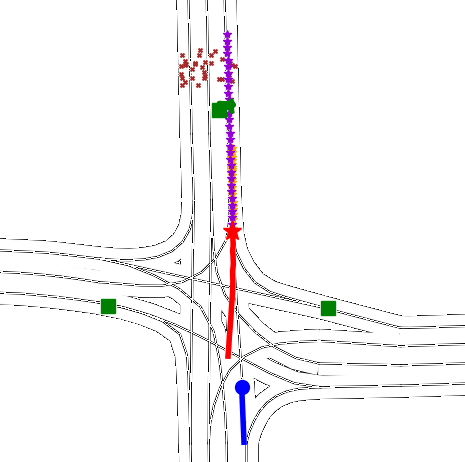
\includegraphics[width=0.32\linewidth]{chapter_5_GAN/qualitative/128_unimodal.png}} \tabularnewline
	\end{tabular}
	\caption[Qualitative Results using our Attention-based GAN best model (including target points extraction and class balance)]{Qualitative Results using our Attention-based GAN best model (including target points extraction and class balance). The legend is as follows: our vehicle (\textcolor{blue}{ego}), the target \textcolor{red}{agent}, and \textcolor{ForestGreen}{other agents}. We can also see the \textcolor{orange}{real} trajectory, the \textcolor{purple}{prediction} and potential \textcolor{brown}{goal-points}. Markers are current positions.}
	\label{fig:chapter_5_GAN/Unimodal_results}
\end{figure*}

\section{Summary}
\label{sec:5_summary}

Forecasting the future trajectories of surrounding actors in the scene is mandatory to achieve a safe planning, and thus, a crucial part of the Autonomous Driving stack. In this Chapter we explore a \ac{GAN}-based \ac{LSTM} with \ac{MHSA} for unimodal vehicle \ac{MP} using the Argoverse 1 Motion Forecasting Benchmark. Our model considers both the deep physical and social context of the scene to predict the most plausible trajectory using a generative model, and achieves competitive results in comparison to other state-of-the-art methods regarding the case of unimodal prediction. Given the aforementioned results, we realize that this uni-modal method lacks of plausible multi-modality and capacity to model complex traffic scenarios, so the future steps are an enhanced social attention and interaction, high-level and well-structured physical context, specially focusing on the vector features of HD Map, in order to produce feasible and realistic multi-modal trajectories.